% LaTeX source for ``Introduction to Computer Science (Java/Pi Edition)''
% Copyright (c) 2015- David S. Read, All Rights Reserved

\chapter{Raspberry Pi Setup for CS-106}

\index{file}
\index{type!file}

\section{The Raspberry Pi Hardware}

\beforefig
\centerline{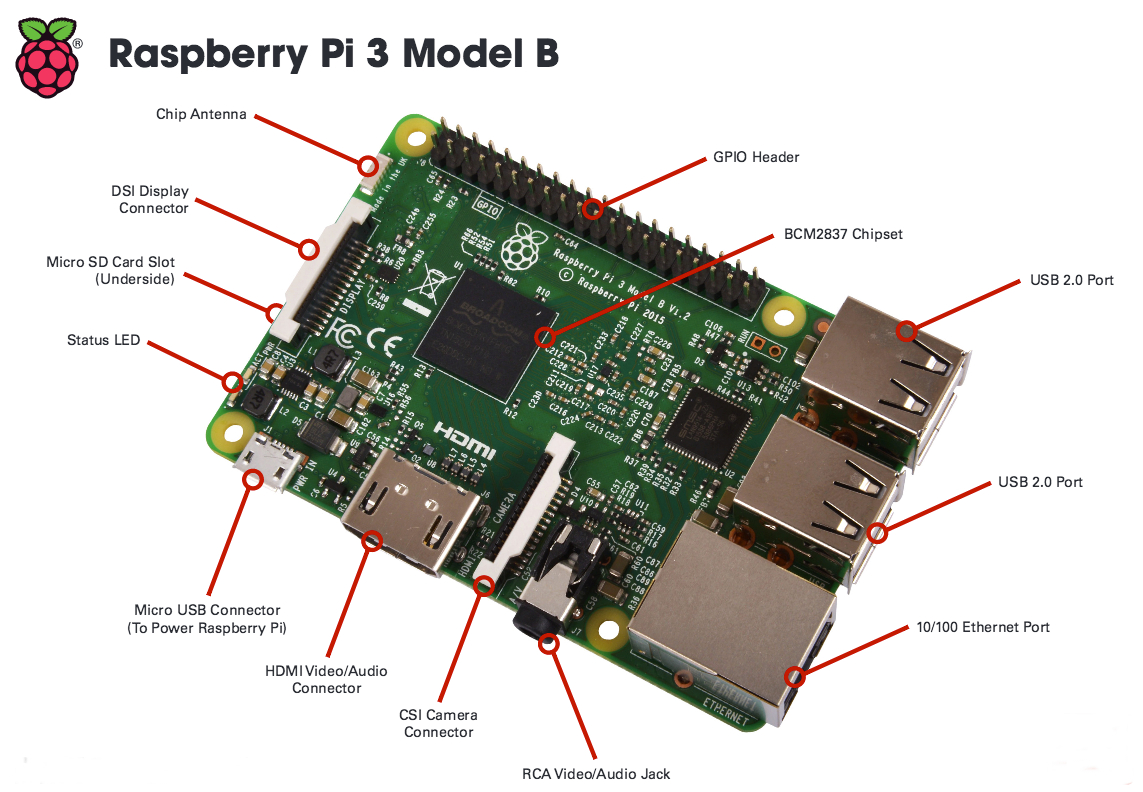
\includegraphics[height=3.50in]{pi_images/Raspi-3-Layout.jpg}}
\afterfig

\index{Raspberry Pi}

Review the image above. All of the major connection points are labeled. We'll be making use of several of these during the setup process.

The Raspberry Pi\footnote{The official website for information on the Raspberry Pi is \url{https://www.raspberrypi.org/}} is a complete computer. It contains all the components of a computer which we cover in the first chapter of this book. Further, it is designed to make it possible to attach a lot of different types of hardware to it.\footnote{See \url{https://www.raspberrypi.org/help/what-is-a-raspberry-pi/} for an overview of the Raspberry Pi}

We generally only connect devices to our computers using commodity interfaces such as USB ports. The Pi lets us make more direct connections into the system. This ability to connect specialized hardware is largely provided by the GPIO header. We'll start working with the GPIO header when we start working on our labs.

For now, you will need to do four things in order to complete the steps outlined in this setup chapter:

\begin{enumerate}
	\item Insert a micro-SD card that has the \textbf{NOOBS} software on it. Your instructor will work through getting that ready for you.
	\item Connect a USB keyboard and mouse
	\item Connect a monitor to the HDMI video port
	\item Connect a power supply to the micro USB port (located next to the HDMI connector)
\end{enumerate}

\textbf{Micro-SD Card} \newline
\beforefig
\centerline{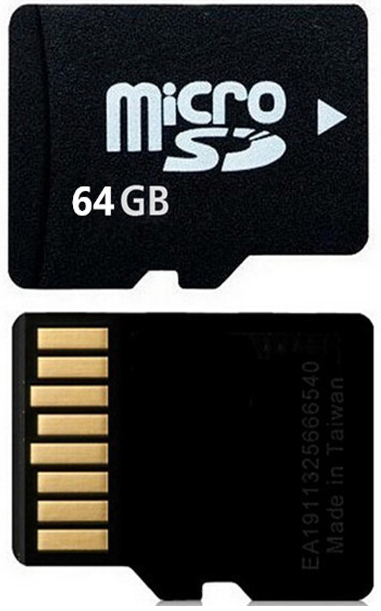
\includegraphics[height=1.50in]{pi_images/micro-sd-card.jpg}}
\afterfig

\index{Micro-SD Card}

The micro-SD card acts as the Pi's disk drive. It houses the operating system as well as user files (such as the programs you write). A minimum size of 8-gigabytes (8GB) is recommended for use with your Pi.

SD cards are manufactured to support different speeds for reading and writing data, known as the card's \textit{transmission speed}. The cards will be marked with a \textbf{class} number.\footnote{The documentation for understanding an SD card's class and managed by the SD Association. See \url{https://www.sdcard.org/developers/overview/speed\_class/}} The class is used to indicate the minimum read and write speed of the card. For example, a class 10 SD card has a minimum transmission speed of 10 megabytes per second while a class 4 SD card has a minimum speed of 4 megabytes per second.

\textbf{\textit{It is recommended that you use a card speed of class 10 or faster for your Pi's SD card.}} Slower cards will have noticeably poorer performance when loading and saving programs and data.

The SD card should have the operating system installer placed on it. The defacto Pi OS installer is called NOOBS (New Out Of Box Software). This is the installer that we will leverage throughout these setup instructions.

Note that the micro-SD card is inserted with the metal connections facing the underside of the Pi. Here is a closeup of a micro-SD card inserted into the Pi. We are looking at the Pi from the bottom. Note that the printed side of the card (side opposite the metal connectors) is facing away from the bottom of the Pi:

\beforefig
\centerline{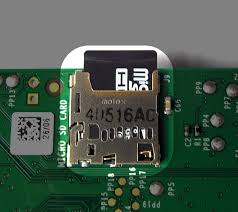
\includegraphics[height=1.0in]{pi_images/micro-sd-insert-into-pi.jpg}}
\afterfig


\textbf{HDMI Connection} \newline
The Pi's default monitor connection uses HDMI. If you are connecting to a monitor that does not support HDMI you will need to use an adapter. Your instructor will have information regarding whether this is necessary in your case.

\index{HDMI}

Connect the HDMI cable (or adapter) to the HDMI port on the Pi and connect the other end to the input for the monitor.

\textbf{Power Supply} \newline
The Pi requires its power be supplied using a micro-USB connection. Most typical USB power supplies (commonly used with cell phones and tablets) should work as long as they use a micro-USB connector.

The Pi does not have a power switch. To turn on the Pi, connect it to a power source. When you are finished with the Pi you should shut down the operating system according to its instructions. Once shutdown, you may disconnect the Pi's power source.

\newcommand{\footnoteref}[1]{\textsuperscript{\ref{#1}}}

\textbf{Software} \newline
The remainder of this chapter will walk through the steps required to setup and install the software required to use the Pi for our class. Some of the steps will take a while to complete since it has to copy a lot of data around on the SD card or download data from various sites in the Internet. Here is an overview of the major tasks and estimate of elapsed time for each step.\footnote{\label{SdClass}These times are based on using a class 10 SD card. Times for slower SD cards will be longer. For example, when using a class 4 SD card the entire installation process took over 3 hours to complete.} \newline

\begin{center}
	\begin{tabular}{ | c | c | p{5cm} | }
		\hline
		\multicolumn{1}{|c|}{\textbf{Step}} & \multicolumn{1}{c|}{\textbf{Duration}} & \multicolumn{1}{c|}{\textbf{Notes}} \\ \hline
		Install the OS & 15 minutes\footnoteref{SdClass} &  \\ \hline
		Configure Raspbian & 5 minutes & \\ \hline
		Update packages & 15 minutes\footnoteref{SdClass} & This may take longer depending on Internet connection speed and the number of updated packages \\ \hline
		Install Eclipse & 20 minutes\footnoteref{SdClass} & This may vary based on Internet connection speed \\ \hline
		Configure Java and PiLib & 5 minutes & \\ \hline		
		Install Chromium & 5 minutes\footnoteref{SdClass} & This may vary based on Internet connection speed \\ \hline	
		\textbf{Total Setup Time} & About an hour\footnoteref{SdClass} & \\ \hline
	\end{tabular}
\end{center}

\section{Installing the Operating System (OS)}

\index{Raspberry Pi setup}
\index{setup!Raspberry Pi}
\index{operating system setup}
\index{Raspian operating system setup}
\index{NOOBS}

Note that the Raspberry Pi's website contains a lot of information regarding setting up the Pi. The following instructions are specific to our use in this class. Much of what is shown here (at least for the initial OS setup) is similar to the instructions you find there.\footnote{See \url{https://www.raspberrypi.org/help/quick-start-guide/} and \url{https://www.raspberrypi.org/help/noobs-setup/} for some background and information on the Pi's setup process}

\begin{enumerate}
	\item \textbf{Verifying the OS}

Once you have NOOBS downloaded onto your micro SD card, insert the micro SD card into the slot on the underside of the Pi. Next you should connect your Pi to a keyboard (USB connector), mouse (USB connector) and monitor (HDMI connector). Finally, boot up your Pi by connecting a power source to the micro-USB port. 

The first time you turn on your Pi you will see a screen that looks like this:

\beforefig
\centerline{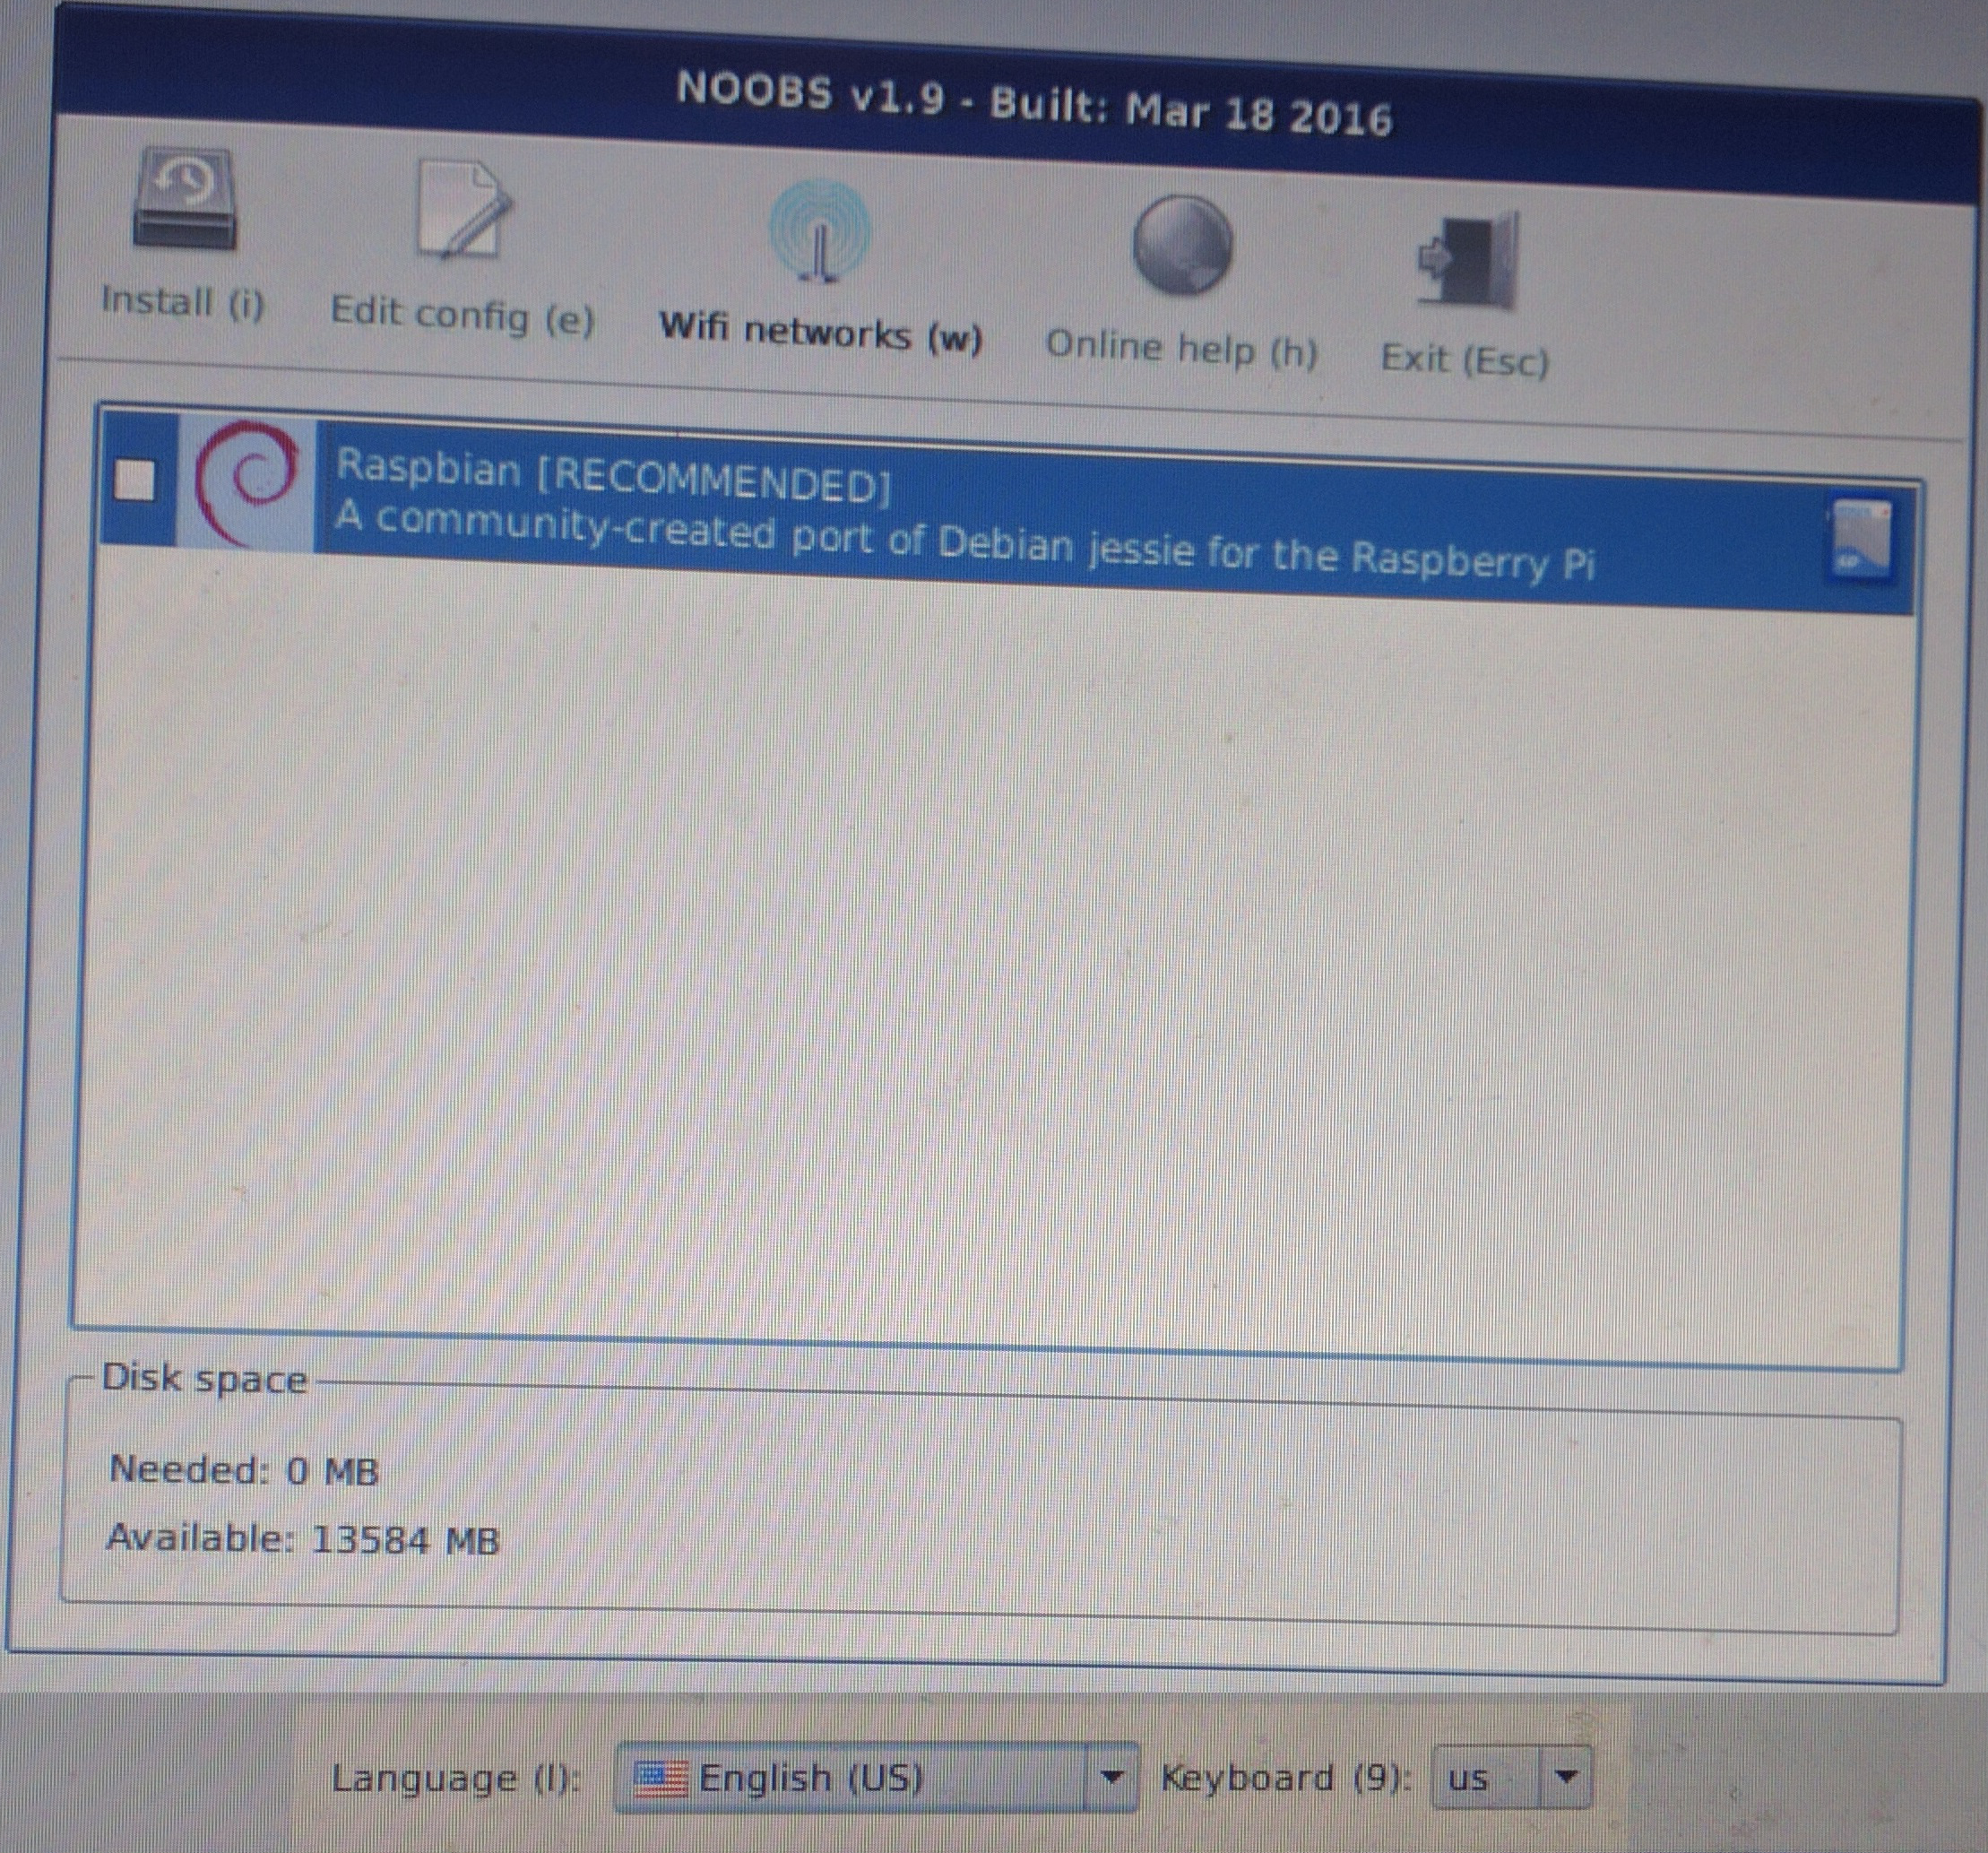
\includegraphics[height=1.75in]{pi_images/setup/OpeningScreen1.jpg}}
\afterfig

On the bottom of the screen you will find the language and keyboard options. Make sure that both the language and keyboard options are set to "US". Next, near the top of the screen, click on the checkbox next to the "Raspbian" option.

\item \textbf{Starting the Installation}

Once that is checked click "Install" in the top-left corner of the window. You should see a dialog pop-up that looks like this:

\beforefig
\centerline{\includegraphics[height=1.75in]{pi_images/setup/OpeningScreen2.jpg}}
\afterfig

On that screen, select "Yes" in order to confirm the installation of Raspbian. \textbf{NOTE:} the installation process will take about 15 minutes\footnoteref{SdClass} to complete.

Once the installation is complete, a dialog will pop up saying that the OS has been installed successfully, click "OK" to finish the installation. 

\beforefig
\centerline{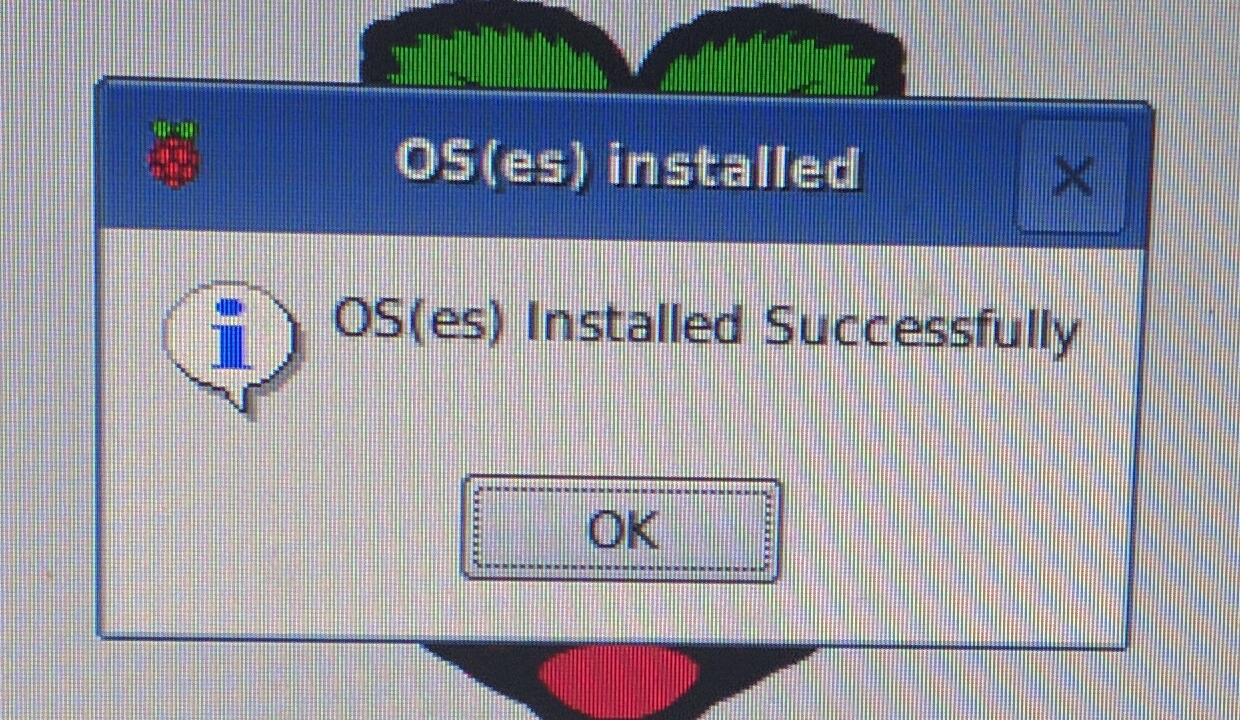
\includegraphics[height=1	in]{pi_images/setup/OpeningScreen3.jpg}}
\afterfig

The Pi will then restart. Once the standard Raspbian graphical desktop opens you may continue.

\end{enumerate}

\section{Configuring your Pi}

\index{configuration!Raspberry Pi}
\index{Raspberry Pi configuration}

\begin{enumerate}
	
	\item \textbf{Connecting to the Internet}

Now that you have your OS installed you need to connect your Pi to the network. Click on the icon in the upper-right of the screen and select the proper network name for your connection.

\beforefig
\centerline{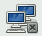
\includegraphics[height=1	in]{pi_images/setup/NoInternet.jpg}}
\afterfig
	
If the network you select requires a password (shared secret) you will be prompted to enter the password. Once the correct password has been entered you will be connected to the network.

Note that some WiFi networks require you to authenticate using a user id and password entered in your browser. To verify that you have an Internet connection open the Epiphany browser (Menu|Internet|Epiphany) and attempt to access a web site.

\item \textbf{Changing the Default Password}

You should now change the password for your Pi to a unique password that only you know.\footnote{The default password for the \texttt{pi} account is \texttt{raspberry}} Open up a terminal window using the terminal icon located with the set of icons in the upper-left corner of the screen:

\index{setting!password}
\index{password!changing}

\beforefig
\centerline{
\includegraphics[height=1 in]{pi_images/setup/Terminal.jpg}}
\afterfig

Once the terminal opens, enter the command \textbf{\texttt{sudo~raspi-config}}. Note that you \textbf{must press the \texttt{Enter}} key after typing a terminal command.\footnote{For the remainder of this setup guide we'll skip the reminder to press the \textbf{Enter} key after typing each command. Just remember it is needed.} After entering the command your screen should look like this:

\beforefig
\centerline{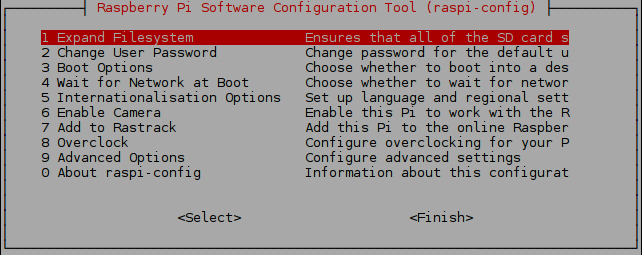
\includegraphics[height=1 in]{pi_images/setup/configuration_tool_menu.jpg}}
\afterfig

This is the main \textbf{Configuration Tool} menu. 

\beforefig
\centerline{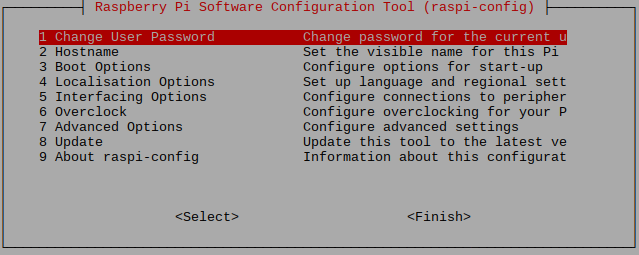
\includegraphics[height=1 in]{pi_images/setup/change_password_choice.png}}
\afterfig


With \textbf{Change User Password} (the first option) selected, press the \textbf{Enter} key. Your screen should now look like this:

\beforefig
\centerline{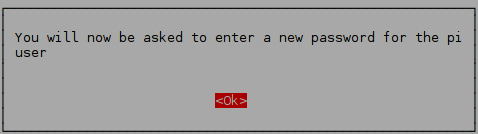
\includegraphics[height=1.0 in]{pi_images/setup/ChangePassword2.jpg}}
\afterfig

Press \textbf{Enter} again to proceed to the password change screen. The screen will return to the terminal prompt which will now prompt you to enter the new password.

As you type your password \textit{you will not see any characters being displayed on the screen.} Press \textbf{Enter} once you have typed your desired password.

\beforefig
\centerline{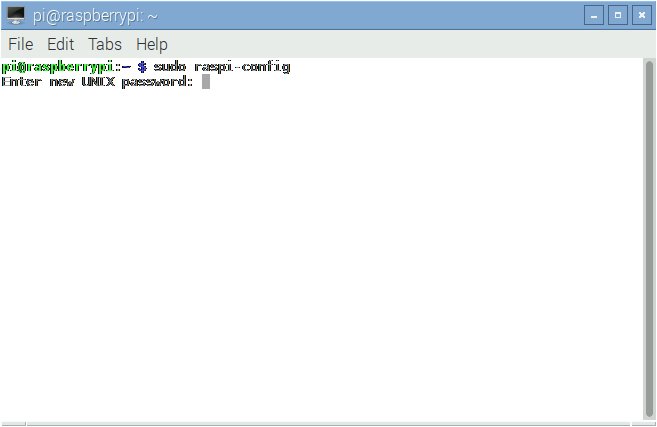
\includegraphics[height=1.5 in]{pi_images/setup/ChangePassword3.jpg}}
\afterfig

You will be prompted to re-enter your password. Once you complete the second password entry, and press \textbf{Enter}, a message will be displayed telling you that your password has been changed. Press \textbf{Enter} one more time and you will be returned to the \textbf{Configuration Tool} menu.

\item \textbf{Setting the Boot Mode}

By default, when the Pi starts up it will launch the graphical environment and log into the \texttt{pi} user account. This means that any user who boots your Pi is logged in, bypassing your password setting. You should change this so that a login screen is presented when the Pi boots.

\index{setting!boot mode}
\index{boot mode!setting}

From the \textbf{Configuration Tool} menu, which should be the current menu after completing the earlier password setting step, use the down arrow to select option three, \textbf{Boot Options}, and press \textbf{Enter}.

\beforefig
\centerline{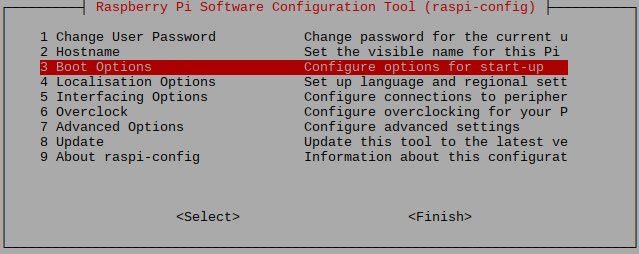
\includegraphics[height=1.5 in]{pi_images/setup/boot_options_choice.png}}
\afterfig

You will be presented with a menu of user interface options. Press \textbf{Enter} to choose the \textbf{B1 Desktop / CLI} option (the first option).

\beforefig
\centerline{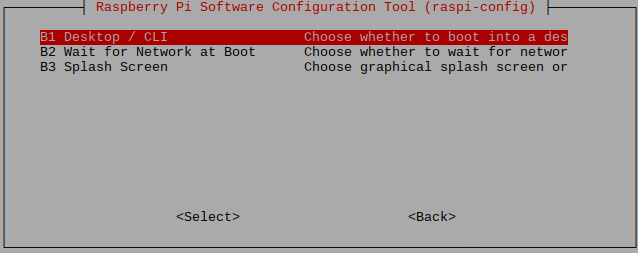
\includegraphics[height=1.5 in]{pi_images/setup/desktop_cli_choice.png}}
\afterfig

\newpage 

Next, use the down arrow to choose the \textbf{B3 Desktop} option and press \textbf{Enter}. This will set the Pi to boot into the graphical environment, presenting a login screen to the user.

\beforefig
\centerline{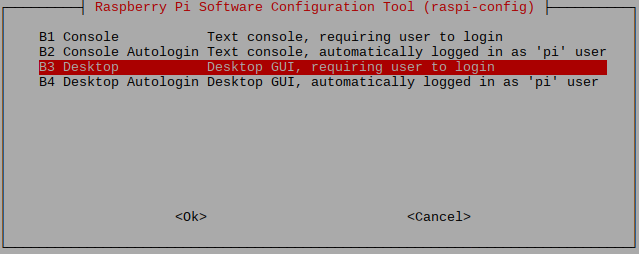
\includegraphics[height=1.0 in]{pi_images/setup/desktop_login_boot_choice.png}}
\afterfig

Again, you will return to the \textbf{Configuration Tool} menu.

% \newpage

\item \textbf{Changing the Locale}

From the \textbf{Configuration Tool} menu use the down arrow to select option four, \textbf{Localisation Options}, and press \textbf{Enter}.

\index{setting!locale}
\index{locale!choosing}

\beforefig
\centerline{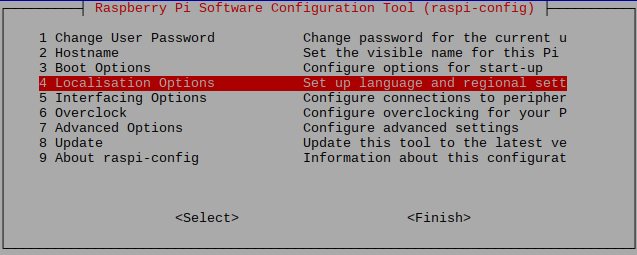
\includegraphics[height=1.5 in]{pi_images/setup/localisation_options_choice.png}}
\afterfig

Next choose the \textbf{Change Locale} option and press \textbf{Enter}.

\beforefig
\centerline{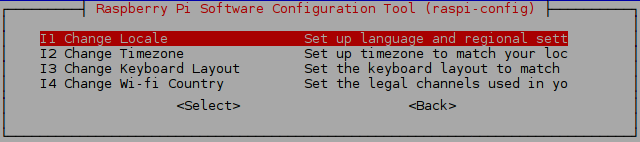
\includegraphics[height=0.75 in]{pi_images/setup/change_locale_choice.png}}
\afterfig

Using the up and down arrow keys scroll through the list of locales and highlight the \textbf{en\_US ISO-8859-1} line. Make sure the item is selected (e.g. shows an asterisk next to the item). You toggle the selection (asterisk) by pressing the spacebar while the line is highlighted.

\beforefig
\centerline{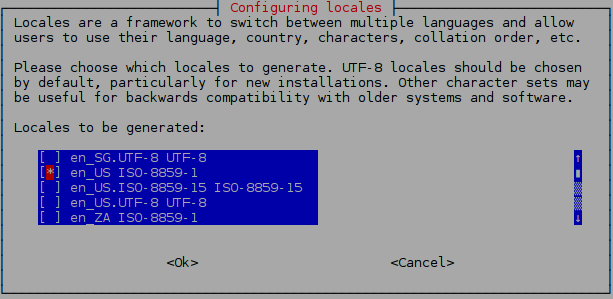
\includegraphics[height=1.5 in]{pi_images/setup/locale_en_us_iso.png}}
\afterfig

Use the \textbf{Tab} key to highlight the \textbf{Ok} option and press the \textbf{Enter} key.

You will then be shown a screen where you choose the default locale. Use the up and down arrow keys to highlight the \textbf{en\_US} option and press \textbf{Enter}.

\beforefig
\centerline{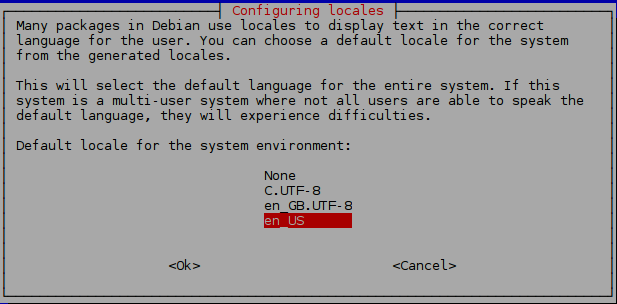
\includegraphics[height=1.5 in]{pi_images/setup/configure_default_locale.png}}
\afterfig

Again, you will return to the \textbf{Configuration Tool} menu.

% \newpage

\item \textbf{Changing the Timezone}

The next step is to set the timezone of your Pi. From the \textbf{Configuration Tool} menu select option four again, \textbf{Localisation Options}, and press \textbf{Enter}. Next, select option \textbf{I2, Change Timezone} and press \textbf{Enter}.

\index{setting!timezone}
\index{timezone!setting}

\beforefig
\centerline{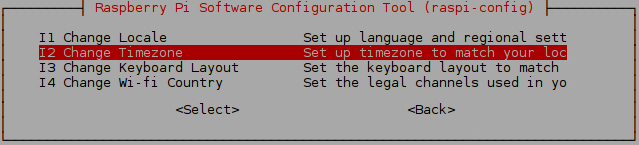
\includegraphics[height=0.75 in]{pi_images/setup/ChangeTimezone1.jpg}}
\afterfig

Use the up and down arrows to navigate to the \textbf{US} option under the \textbf{Geographic area} and press \textbf{Enter}.

\beforefig
\centerline{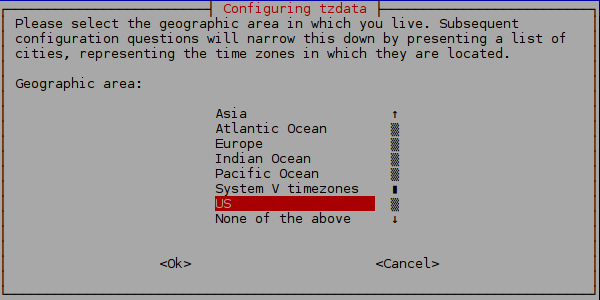
\includegraphics[height=1.5 in]{pi_images/setup/ChangeTimezone2.jpg}}
\afterfig

Next, select the \textbf{Eastern} option under the \textbf{Time zone} and press \textbf{Enter}.

\beforefig
\centerline{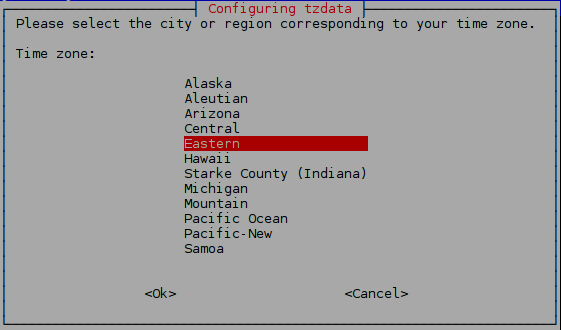
\includegraphics[height=1.5 in]{pi_images/setup/ChangeTimezone3.jpg}}
\afterfig

\newpage

\item \textbf{Changing the Keyboard Layout}

The next step is to set the keyboard layout for your Pi. From the same menu screen select option four again, \textbf{Localisation Options}, and press \textbf{Enter}. Next, select option \textbf{I3, Change Keyboard Layout} and press \textbf{Enter}.

\index{setting!keyboard layout}
\index{keyboard layout!setting}

\beforefig
\centerline{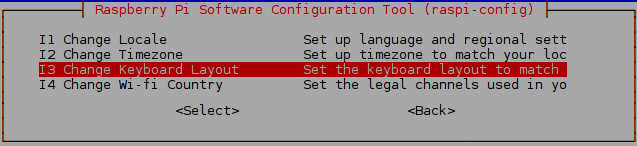
\includegraphics[height=0.75 in]{pi_images/setup/change_keyboard_layout_choice.png}}
\afterfig

% \newpage

Using the up and down arrow keys select the \textbf{Generic 104-key PC} option and press \textbf{Enter}.

\beforefig
\centerline{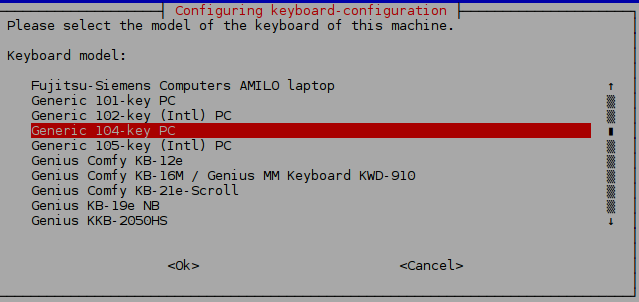
\includegraphics[height=1.5 in]{pi_images/setup/keyboard_choice_generic.png}}
\afterfig

You will be asked to choose the keyboard layout language. Use the up and down arrows to select the \textbf{English (US)} option and press \textbf{Enter}.

\beforefig
\centerline{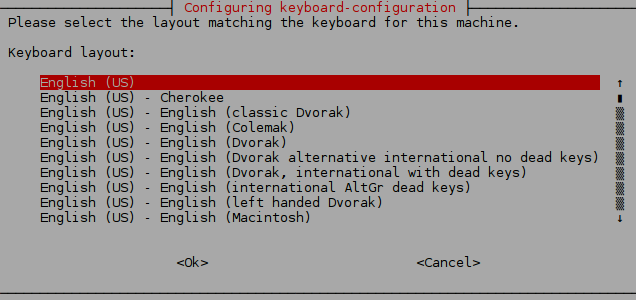
\includegraphics[height=1.5 in]{pi_images/setup/keyboard_language_choice_english.png}}
\afterfig

You will then be asked to configure the \textit{AltGr} setting. Using the up and down arrows choose the \textbf{The default for the keyboard layout} option and press \textbf{Enter}.

\beforefig
\centerline{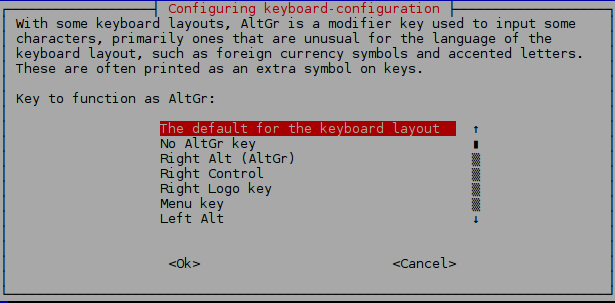
\includegraphics[height=1.5 in]{pi_images/setup/keyboard_layout_choice_default_altgr.png}}
\afterfig

Next you will be asked to configure the \textit{Compose key} setting. Using the up and down arrows choose the \textbf{No compose key} option and press \textbf{Enter}.

\beforefig
\centerline{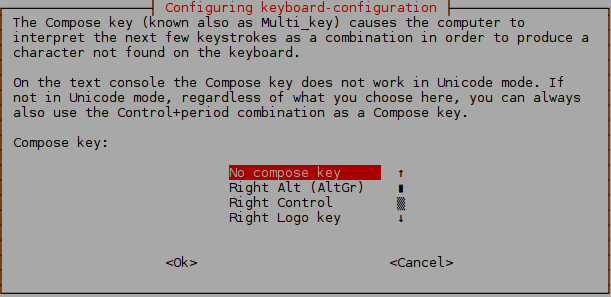
\includegraphics[height=1.5 in]{pi_images/setup/keyboard_layout_default_compose_key.png}}
\afterfig

Finally you will be asked whether you want to enable the \textit{Ctrl-Alt-Backspace key combination} function. Using the \textbf{Tab} key select the \textbf{No} option and press the \textbf{Enter} key.

\beforefig
\centerline{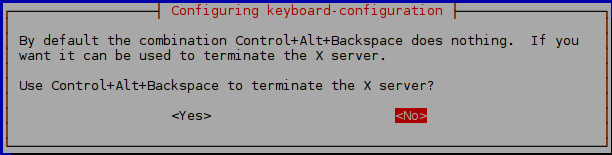
\includegraphics[height=0.75 in]{pi_images/setup/keyboard_layout_default_altctlbksp.png}}
\afterfig

You will be brought back to the \textbf{Configuration Tool} menu again. You may exit the menu by using the \textbf{Tab} key to select the \textbf{Finish} option and pressing \textbf{Enter}. 

\textit{If you changed the boot option as suggested in an earlier step} you will be asked whether or not the Pi should be rebooted. If asked, you may use the \textbf{Tab} key to choose the \textbf{No} option and press the \textbf{Enter} key.

\beforefig
\centerline{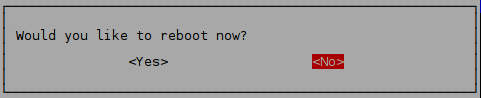
\includegraphics[height=0.75 in]{pi_images/setup/reboot_request_screen.jpg}}
\afterfig

At this point you will return to the terminal prompt.

\item \textbf{Updating the Packages}

Now we need to update several packages on the Pi. These packages represent programs that are installed on the Pi as part of the NOOBS setup process but may have been updated since the NOOBS installer was created.

\index{updating system packages}
\index{system updates}

Enter the command \textbf{\texttt{sudo~apt-get~update}} into the terminal. This process will take a couple of minutes to run.

\beforefig
\centerline{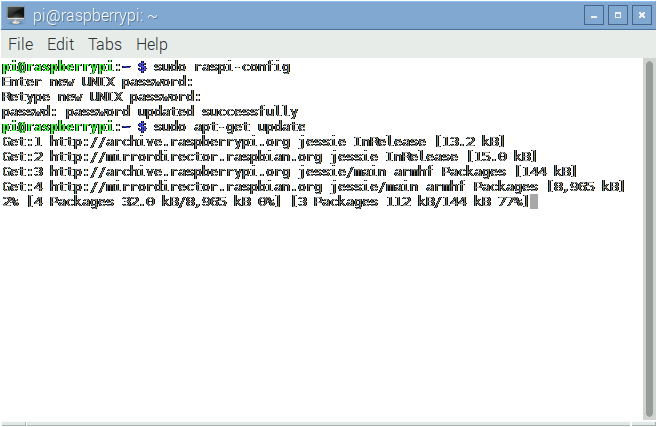
\includegraphics[height=1.5 in]{pi_images/setup/UpdatePackages1.jpg}}
\afterfig

\newpage

Next, enter the command \textbf{\texttt{sudo~apt-get~upgrade}} into the terminal. You will be asked if you want to continue the upgrade. Type the letter \textbf{\texttt{Y}} and press the \textbf{Enter} key to continue.  \textit{This process may take 15 minutes or more to complete depending on your Internet connection speed.}\footnoteref{SdClass}

\beforefig
\centerline{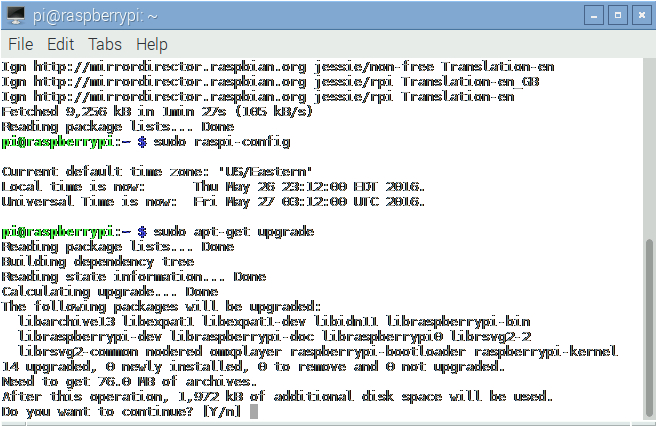
\includegraphics[height=1.5 in]{pi_images/setup/UpdatePackages2.jpg}}
\afterfig

\item \textbf{Installing Eclipse}

\index{Eclipse installation}

A popular Java Integrated Development Environment (IDE) is Eclipse. To install Eclipse enter the command \textbf{\texttt{sudo~apt-get~install~eclipse}} on the terminal's command line. Again, you will be asked if you want to continue, and again you will type the letter \textbf{\texttt{Y}} and press the \textbf{Enter} key to continue. This step may take 20 minutes or more\footnoteref{SdClass} to complete.

\index{Eclipse!installation}
\index{install!Eclipse}

\beforefig
\centerline{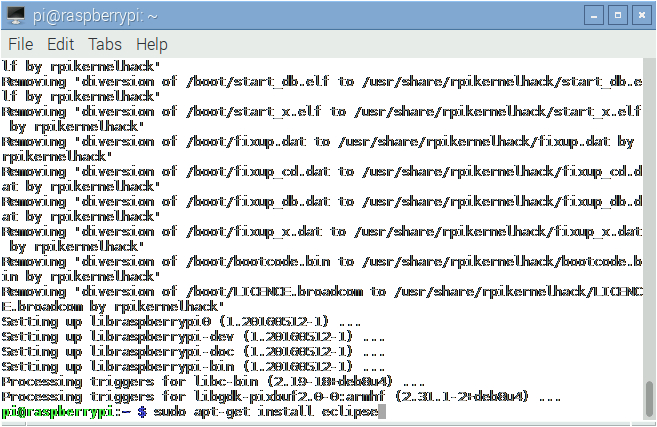
\includegraphics[height=1.5 in]{pi_images/setup/UpdatePackages3.jpg}}
\afterfig

\item \textbf{Configuring Java}

To setup the proper Java compiler, enter the command \textbf{\texttt{sudo~update-alternatives~--config~javac}} and then enter the number next to the option containing the term \textbf{oracle}. In the example shown below this is option number 2.

\beforefig
\centerline{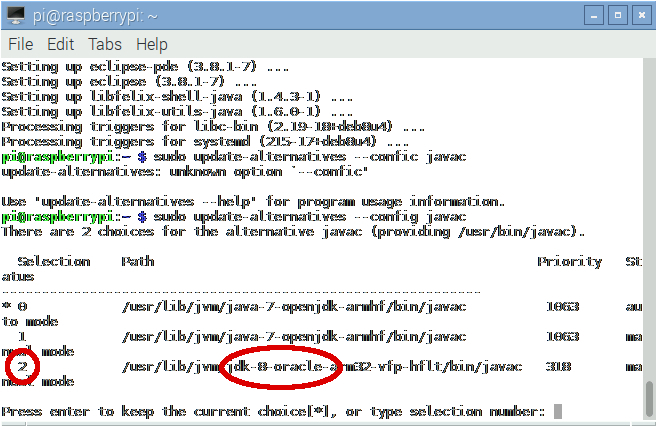
\includegraphics[height=1.5 in]{pi_images/setup/UpdatePackages4.jpg}}
\afterfig

To setup the proper Java runtime, enter the command \textbf{\texttt{sudo~update-alternatives~--config~java}} and again, enter the number next to the option containing the term \textbf{oracle}. In the example shown below this is option number 2.

\beforefig
\centerline{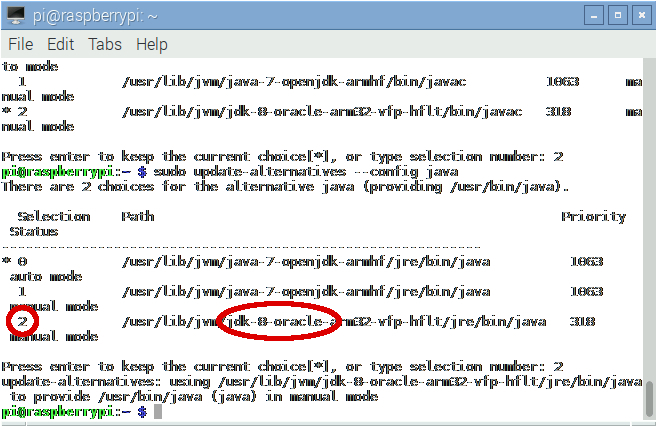
\includegraphics[height=1.5 in]{pi_images/setup/UpdatePackages5.jpg}}
\afterfig

%\item \textbf{Java-GPIO Setup Script}

%At this point your instructor will provide you with a script to be run that creates a Java configuration that will allow you to run Java programs %that use the GPIO header. Refer to the information from you instructor to complete this step.

\end{enumerate}

\iffalse % Comment out this section since there is no need to run Java as root for PiLib anymore

\section{Configuring Eclipse}

Now we will configure Eclipse. First open Eclipse, which can be found under the Programming section of the Pi menu.

\index{Eclipse!configuration}
\index{configure!Eclipse}

\beforefig
\centerline{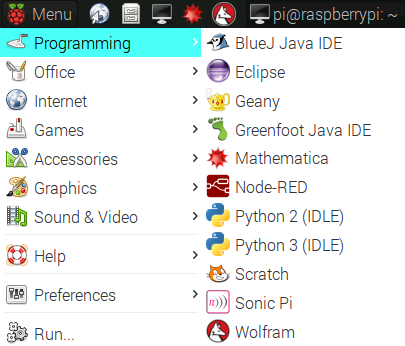
\includegraphics[height=2.5 in]{pi_images/setup/ConfigureEclipse1.jpg}}
\afterfig

Once Eclipse opens, you will be asked which Workspace you would like to use. The default workspace is what we will be using, so just click \textbf{OK} to continue.

\beforefig
\centerline{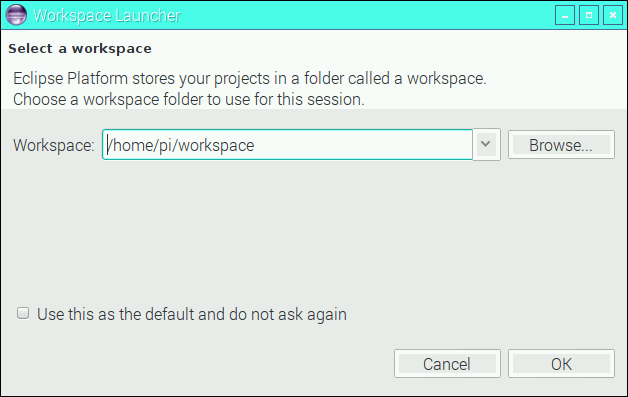
\includegraphics[height=2.5 in]{pi_images/setup/ConfigureEclipse2.jpg}}
\afterfig

Next, click on the \textbf{Workbench} option to continue to Eclipse's Java workbench.

\beforefig
\centerline{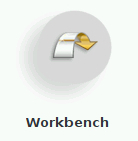
\includegraphics[height=1.5 in]{pi_images/setup/ConfigureEclipse3.jpg}}
\afterfig

Under the \textbf{Window} menu, click on the \textbf{Preferences} option on the bottom.

\beforefig
\centerline{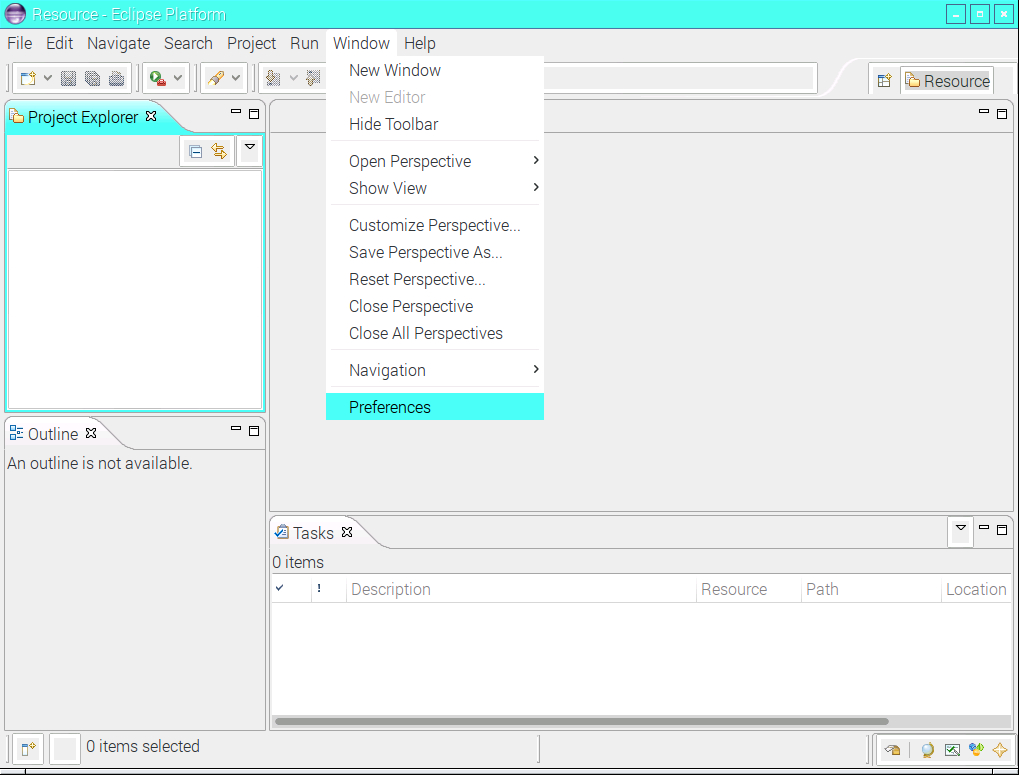
\includegraphics[height=3.0 in]{pi_images/setup/ConfigureEclipse4.jpg}}
\afterfig

Expand the \textbf{Java} selection by clicking the plus sign \textbf{+} next to it, and select the \textbf{Installed JREs} option. Select the \textbf{jdk-8-oracle} JRE and click the \textbf{Duplicate} button.

\beforefig
\centerline{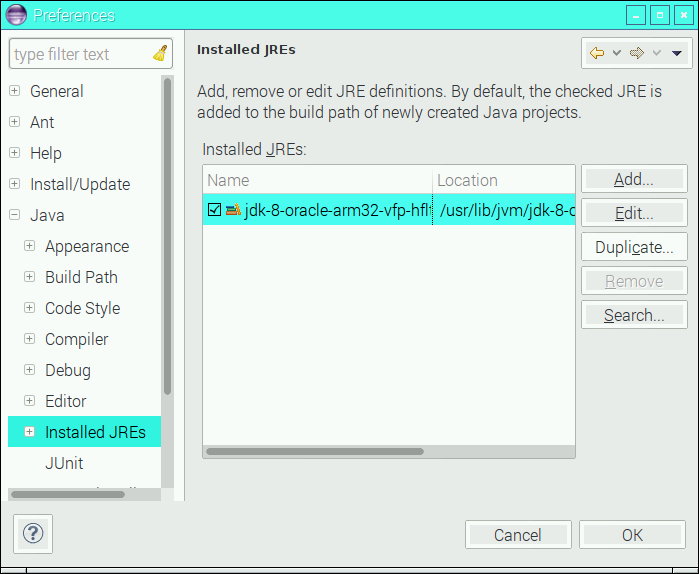
\includegraphics[height=3.0 in]{pi_images/setup/ConfigureEclipse5.jpg}}
\afterfig

A screen will pop up allowing you to edit the JRE definition before you create the duplicate. Change the \textbf{JRE name:} by removing the \textbf{(1)} (including the space) and appending \textbf{\texttt{-root}}. Next, under the \textbf{Default VM arguments}, add \textbf{\texttt{--run-as-root}}. Verify your changes by comparing them to the screenshot below:

\beforefig
\centerline{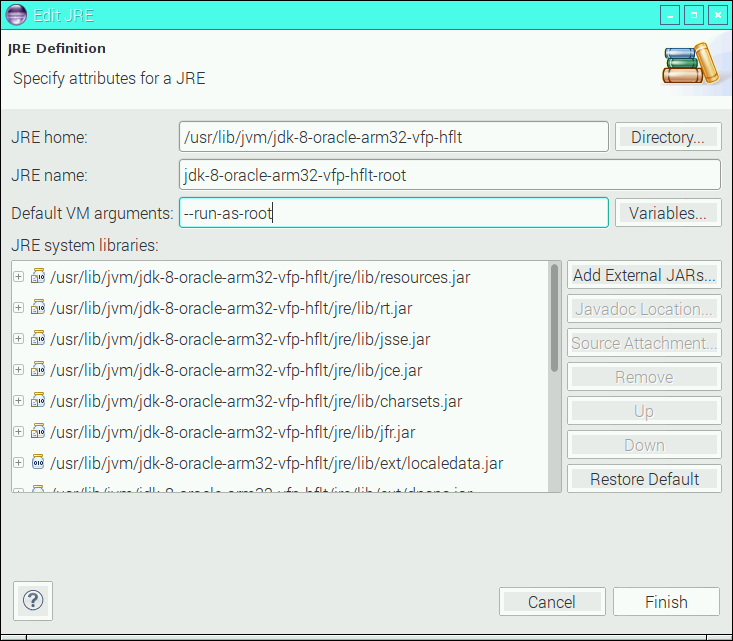
\includegraphics[height=3.0 in]{pi_images/setup/ConfigureEclipse6.jpg}}
\afterfig

Click the \textbf{Finish} button and make sure that the checkbox next to the JRE that you just created (with the name ending with -root) is not checked. To complete the process and click the \textbf{OK} button.

\beforefig
\centerline{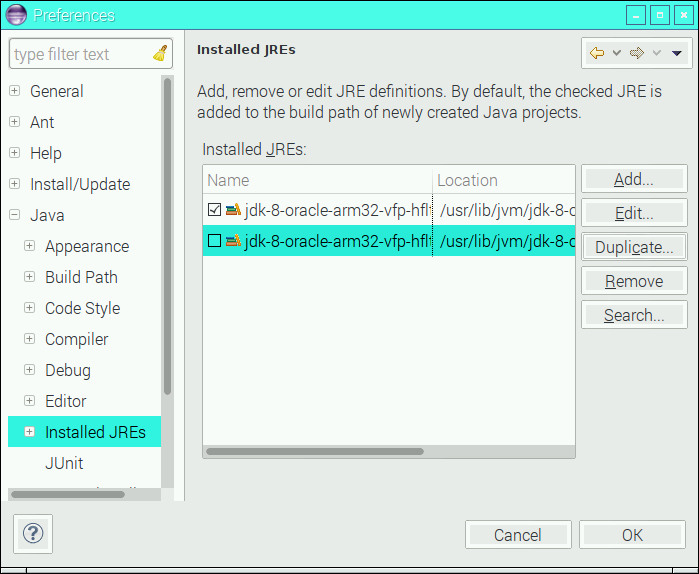
\includegraphics[height=2.5 in]{pi_images/setup/ConfigureEclipse7.jpg}}
\afterfig

\fi % Comment out this section since there is no need to run Java as root for PiLib anymore

%\newpage

\section{Setup the PiLib Server}\label{setupPiLibServer}

\index{PiLib}
\index{library!PiLib}
\index{PiLib!Server program}

To simplify working with the GPIO interface and breadboard components we will use a library, \textbf{PiLib}, that provides two features:

\index{PiLib server!installation}
\index{install!PiLib server}

\begin{enumerate}
	\item Allows a library of functions available to our Java program to control the LEDs and react to the buttons being pressed
	\item Provides a web-based view of the current GPIO operations. This allows you to view the configured LEDs and buttons as well as see each LED's state (on/blink/off) and interact with buttons (by pressing them via a mouse click) 
\end{enumerate}

The PiLib library is made up of two parts, the server program and the client library. The client library will be included in each lab and will be described in the lab appendix. The server has to be installed on your Pi and then started each time you want to run a program that uses the client library to interact with the breadboard (LEDs and buttons).

Your instructor will give you the address of a website to download the \textbf{\texttt{PiLibServerDist.tar.gz}} file. I recommend for convenience you place that file in your home directory. Once you've placed the file in your home directory, access a terminal and type the following commands:

\texttt{\$ cd} \linebreak
\texttt{\$ tar xvzf PiLibServerDist.tar.gz}

\textit{Note that the} \texttt{\$} \textit{(dollar sign) is the terminal prompt.} You do not type the \texttt{\$}. Also, your terminal prompt may look different than a plain dollar sign.

The first command (\texttt{cd}) assures your terminal is accessing your home directory. You don't need to type the first command if your terminal automatically opens in your home directory.

The second command will create a directory called \textbf{\texttt{PiLibServerDist}} that contains the server program and a script to run it.

See the section \textbf{\textit{Starting the PiLib Server}} in the labs appendix for information on using the PiLib Server.

\section{Your Pi Is Configured}

\textbf{Congratulations!} Your Pi is now setup with an up-to-date operating system and configured so that it is ready for you to complete the course labs.

\index{Login screen}

Remember that the next time you start up your Pi it will prompt you for a login id and password. The login account name, unless you change it, is \textbf{\texttt{pi}}. The password is whatever you set it to earlier in this setup process. (If you don't change it, the default password is \texttt{raspberry})

Here is what the login screen looks like:

\beforefig
\centerline{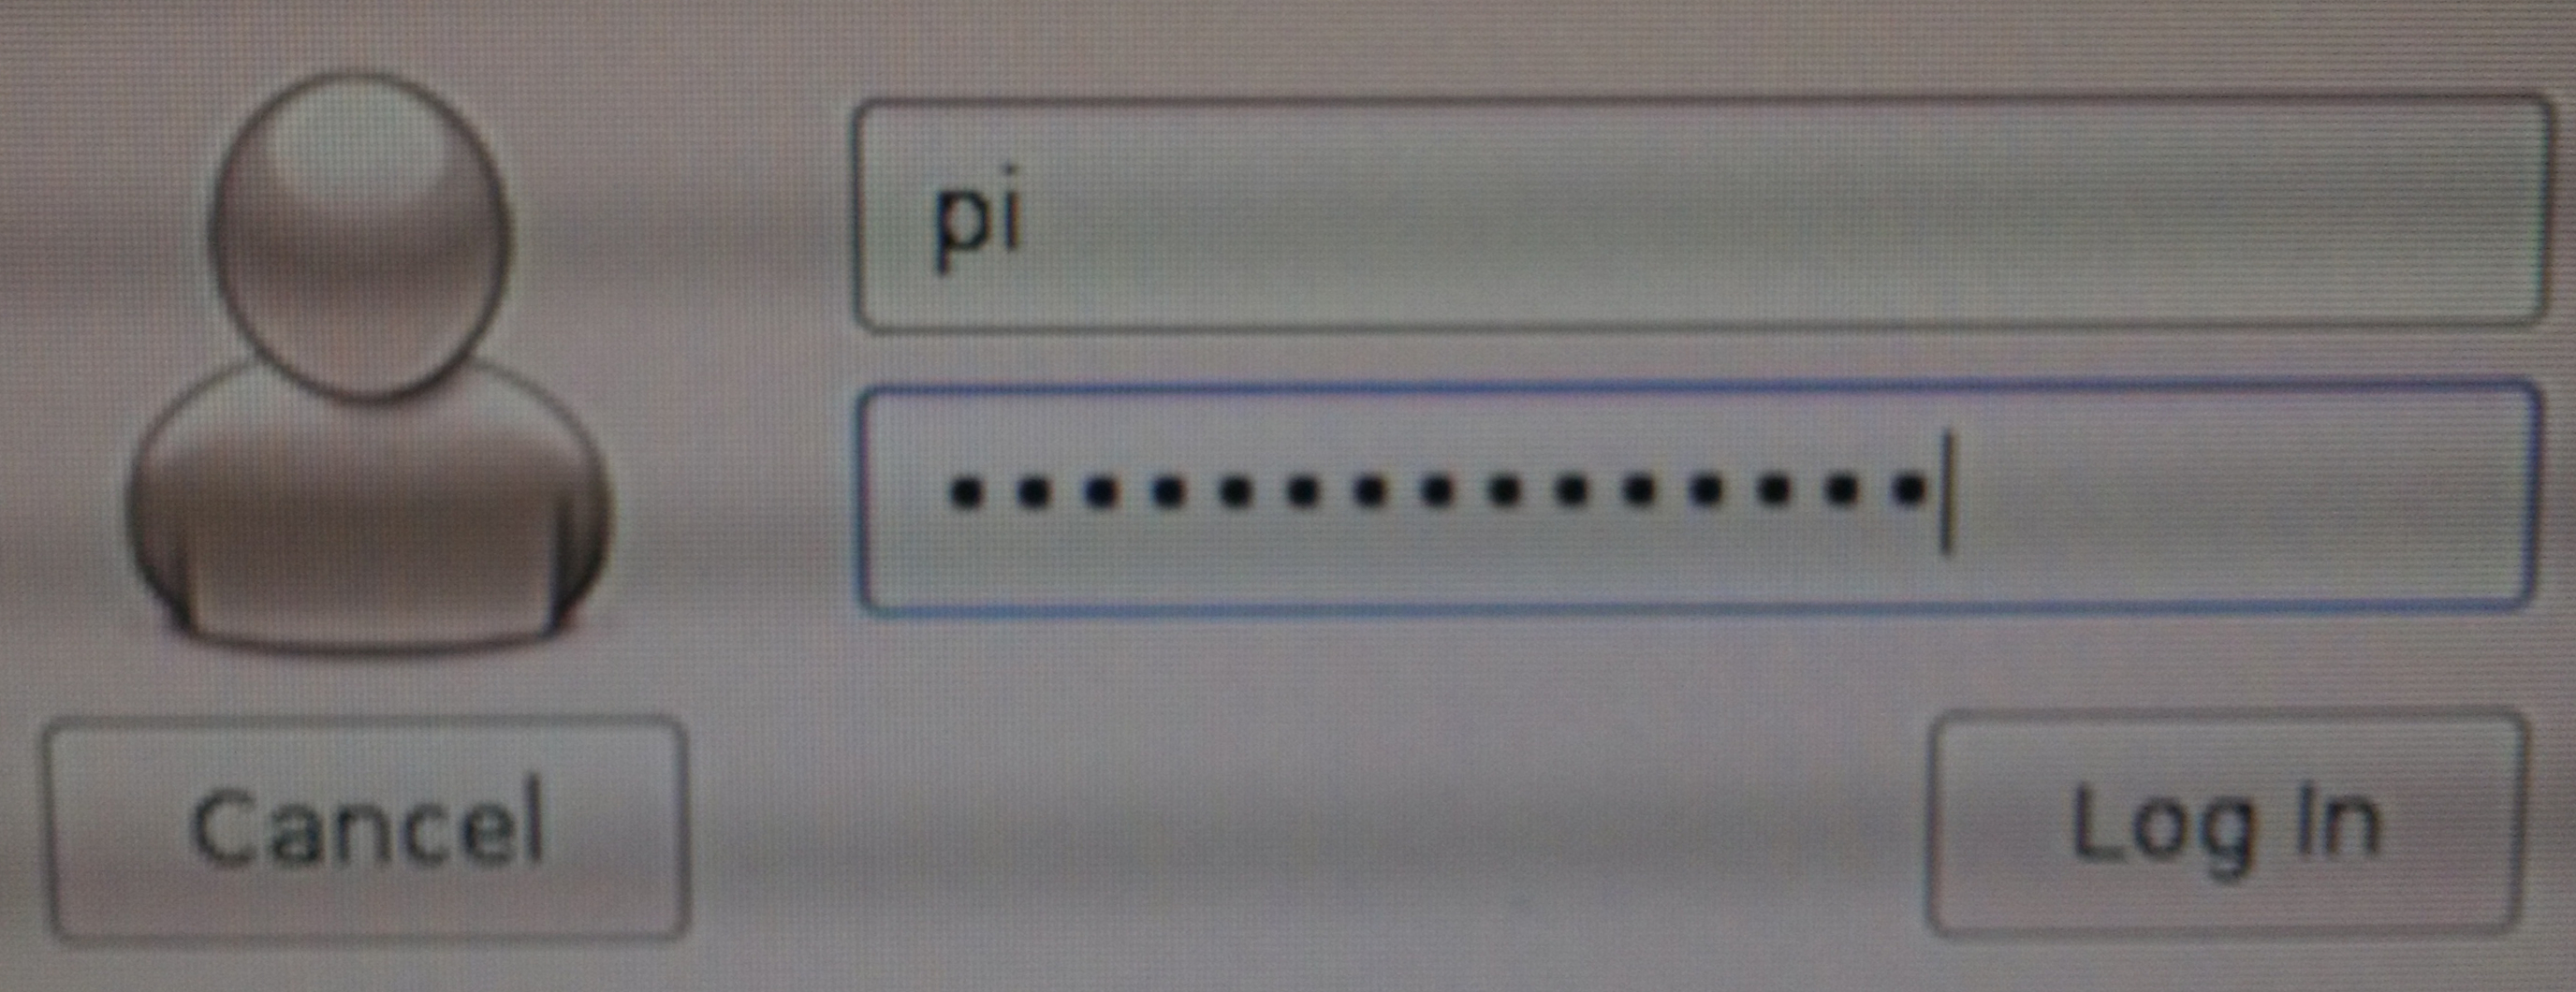
\includegraphics[height=1.0 in]{pi_images/setup/login_screen.jpg}}
\afterfig

Fill in the user id and password then press \textbf{\texttt{Log In}} and you will see the graphical desktop.